\documentclass[12pt]{scrartcl}
\usepackage[T1]{fontenc}
\usepackage[utf8]{inputenc}
\usepackage[english]{babel}
\usepackage{lmodern}
\usepackage{geometry}
\geometry{a4paper, margin=1in}
\setlength\parindent{0pt}
\usepackage{amsmath,amssymb}
\usepackage{graphicx}
\usepackage{svg}
\usepackage{pdfpages}
\usepackage[colorlinks=true, linkcolor=black, urlcolor=blue, citecolor=black]{hyperref}
\usepackage{listings}
\lstset{
  basicstyle=\ttfamily\small,
  frame=single,
  numbers=left,
  numberstyle=\tiny,
  breaklines=true,
  tabsize=2
}
\usepackage[numbers]{natbib}

% Meta
\newcommand{\thesistitle}{Data-driven camera calibration for light field camera systems}
\newcommand{\authorname}{Youssef Daoudi El Boukhrissi}
\newcommand{\matriculation}{4277022}
\newcommand{\supervisor}{Prof.\ Dr.\ J{\"u}rgen Hesser}
\newcommand{\university}{Heidelberg University}
\newcommand{\submissiondate}{28.02.2026}
\newcommand{\authormail}{youssefdaoudi275@gmail.com}

\begin{document}

% =========================================================
% Title Page
% =========================================================
\begin{titlepage}
\thispagestyle{empty}

\begin{center}
    \vspace*{2.5cm}

    {\large \textbf{University of Heidelberg}\par}
    \vspace{0.3cm}
    {\large \textbf{Faculty of Mathematics and Computer Science}\par}
    \vspace{0.15cm}
    {\large \textbf{Institute of Computer Science}\par}
    \vspace{0.15cm}
    {\large \textbf{Research Group: Data Analysis and Modeling in Medicine}\par}

    \vspace{2.2cm}

    {\large Bachelor's Thesis in Computer Science\par}

    \vspace{2.4cm}

    {\LARGE\bfseries Data-driven camera calibration\par}
    \vspace{0.3cm}
    {\LARGE\bfseries for light field camera systems\par}
\end{center}

\vfill
\begin{flushleft}
Name: Youssef Daoudi El Boukhrissi\\
Student ID: 4277022\\
Supervisor: Prof.\ Dr.\ Jürgen Hesser\\
Submission date: 28 February 2026
\end{flushleft}

\end{titlepage}
\pagenumbering{gobble}


% =========================================================
% Abstract
% =========================================================
\section*{Abstract}
% Write later
\cleardoublepage

% =========================================================
% TOC
% =========================================================
\tableofcontents
\clearpage

% =========================================================
% figures
% =========================================================
\listoffigures
\clearpage

\pagenumbering{arabic}

% =========================================================
% Chapter 1: Introduction
% =========================================================
\section{Introduction}

\subsection{Motivation}
% General relevance of camera calibration
% Importance for computer vision and light field systems

\subsection{Challenges and Problem Statement}
% Existing challenges and open issues
% Limitations of classical calibration
% Practical problems in long-term and real-world setups

\subsection{Research Questions}

The following research questions guide this thesis:

\begin{itemize}
  \item \textbf{RQ1:} Can the target-free calibration method LiFCal be used to automatically calibrate a multi-camera light field system without human interaction or the use of a checkerboard?

  \item \textbf{RQ2:} How well does LiFCal perform when calibrating a multi-camera light field system, and can it replace a classical checkerboard-based calibration?

  \item \textbf{RQ3:} Under which conditions and requirements can an automatic, target-free recalibration of a multi-camera light field system be successfully performed?
\end{itemize}

\subsection{Structure of the Thesis}
% Brief overview of all chapters

\clearpage

% =========================================================
% Chapter 2: Theoretical Background
% =========================================================
\section{Theoretical Background}

% Chapter 2.1 Pinhole Camera Model
\subsection{Pinhole Camera Model}

Cameras are the primary devices used to capture visual
information from the real world into an image. To process and analyze this information
computationally, it is necessary to describe the imaging process using a 
camera model \cite{StanfordCS231ACameraModels}.

\begin{figure}[htbp]
    \centering
    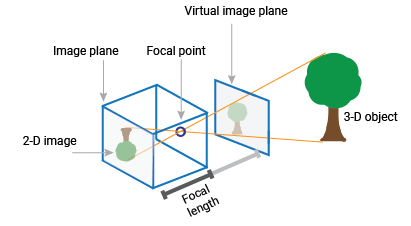
\includegraphics[width=0.8\textwidth]{figures/Pinhole-Camera.png}
    \caption{Illustration of the pinhole camera model. Source: \cite{MathWorksCameraCalibration}.}
    \label{fig:pinhole_camera_model}
\end{figure}

The pinhole camera model describes a simple imaging system in which light rays
from a 3D scene pass through a small aperture and are projected through the focal point
onto a 2D image plane \cite{StanfordCS231ACameraModels}. The aperture limits the incoming light such
that each point in the scene is mapped to a single point on the image plane. In this model,
the projected image is inverted due to the geometry of the projection, as shown in
\autoref{fig:pinhole_camera_model}.
\vspace{0.2cm}

To define the mapping from 3D world coordinates to 2D image coordinates,
the model is mathematically described using two types of parameters \cite{MathWorksCameraCalibration}.

\vspace{0.2cm}
\begin{itemize}
  \item \textbf{Intrinsic Parameters: \hspace{6mm}} 
  \[
  K = 
  \begin{bmatrix}
  f_x & s & c_x \\
  0 & f_y & c_y \\
  0 & 0 & 1
  \end{bmatrix}
  \] 
  
  \vspace{0.3cm}
  where $(f_x, f_y)$ are the focal lengths in pixel units along the x and y axes,
  $s$ is the skew coefficient between the axes, and $(c_x, c_y)$ is the principal point (optical center) in pixel coordinates.
  $K$ is also known as the camera matrix.

  \item \textbf{Extrinsic Parameters:} 
  \[
  [R \mid t] = 
  \begin{bmatrix}
  r_{11} & r_{12} & r_{13} & t_x \\
  r_{21} & r_{22} & r_{23} & t_y \\
  r_{31} & r_{32} & r_{33} & t_z
  \end{bmatrix}
  \]

  \vspace{0.3cm}
  where $R$ is a $3 \times 3$ rotation matrix representing the orientation of the camera
  with respect to the world coordinate system, and $t$ is a $3 \times 1$ translation vector
  representing the position of the camera center in world coordinates.
\end{itemize}

These parameters form the basis of camera calibration, which aims to estimate them accurately.
Also note that in practice, cameras use lenses to focus light onto the image sensor,
which introduces distortions not accounted for in the idealized pinhole model.

% Chapter 2.2 Lens Distortion
\subsection{Lens Distortion}


% Chapter 2.2.1 Radial Distortion
\subsubsection{Radial Distortion}

% Chapter 2.2.2 Radial Distortion
\subsubsection{Tangential Distortion}

% Chapter 2.3 Camera Calibration
\subsection{Camera Calibration}

% 2.3.1 Calibration Parameters and Error Metrics
\subsubsection{Calibration Parameters and Error Metrics}
% Intrinsics, extrinsics, reprojection error

% 2.3.2 Target-Based Camera Calibration
\subsubsection{Target-Based Camera Calibration}
% Checkerboard-based calibration (OpenCV)

% 2.3.3 Bundle Adjustment
\subsubsection{Bundle Adjustment}
% Joint optimization of camera parameters and structure

% 2.4 Light Field Cameras Systems
\subsection{Light Field Camera Systems}

% 2.4.1 Multi-Camera Light Field Systems
\subsubsection{Multi-Camera Light Field Systems}
% Camera arrays (e.g. cross-shaped setup with 13 cameras)

% 2.4.2 Micro-Lens-Array-Based Light Field Cameras
\subsubsection{Micro-Lens-Array-Based Light Field Cameras}
% MLA-based systems as used in LiFCal

% 2.5 State of the Art in Light Field Camera Calibration
\subsection{State of the Art in Light Field Camera Calibration}

\clearpage

% =========================================================
% Chapter Three: Material and Method
% =========================================================
\section{Material and Method}

% ---------------------------------------------------------
% 3.1 Material
% ---------------------------------------------------------
\subsection{Material}

\subsubsection{Synthetic Data Generation with Blender}
% Blender-based scene setup
% Camera array geometry
% Pose variation
% Motivation for synthetic data and reproducibility

\subsubsection{Image Sets and Ground Truth Definition}
% Image set structure
% Naming conventions
% Pose sampling
% Ground truth availability

\subsubsection{Runtime Environment and Toolchain}
% Operating system
% Programming language and libraries
% External tools (OpenCV, LiFCal)
% Custom scripts and execution workflow

% ---------------------------------------------------------
% 3.2 Method
% ---------------------------------------------------------
\subsection{Method}

\subsubsection{Use Case Description}
% Overall system workflow
% Initial calibration, health monitoring, recalibration phases

\subsubsection{Requirements Analysis}
% Functional requirements
% Non-functional requirements
% Traceability to implementation

\subsubsection{UML Class Diagram}
% Main software components
% Responsibilities and relationships

\subsubsection{Health Monitoring and Decision Metrics}
% Health score computation
% Initial calibration health
% LiFCal-based health
% Acceptance and rollback logic

\subsubsection{State Diagram}
% System states
% Transitions between calibration phases
% Periodic execution and decision flow

\clearpage

% =========================================================
% Chapter 4: Results and Evaluation
% =========================================================
\section{Results and Evaluation}

\subsection{Results of Initial Calibration}

\subsubsection{Intrinsic Accuracy}
% fx, fy deviation
% cx, cy deviation

\subsubsection{Extrinsic Accuracy}
% 3D camera positions
% Translation error per camera
% Rotation error per camera

\subsubsection{Reprojection and RMS Error}
% RMS and reprojection error per camera


\subsection{Results of LiFCal-Based Recalibration}

\subsubsection{Reprojection Error after LiFCal}

\subsubsection{Health Score Evolution}
% Health score before/after LiFCal
% Comparison to baseline
\clearpage

% =========================================================
% Chapter 5: Discussion of the Results
% =========================================================
\section{Discussion of the Results}

\subsection{Interpretation of Initial Calibration Results}
% Why errors are low
% Role of checkerboard + ground truth
% Stability across cameras

\subsection{Limitations of LiFCal in the Given Setup}
% Camera type mismatch
% Dependence on depth maps
% Synthetic vs real assumptions

\subsection{Comparison between Initial Calibration and LiFCal}
% What improves
% What degrades
% What cannot be compared fairly

\subsection{Comparison to state of the Art}

\subsection{Potential Extensions and Improvements}
\clearpage

% =========================================================
% Chapter 6: Conclusion and Outlook
% =========================================================
\section{Conclusion and Outlook}

\subsection{Conclusion}
% What was implemented
% What worked well
% What was learned

\subsection{Outlook}
% Real hardware LF camera
% Better depth estimation
% Alternative target-free methods

% =========================================================
% Appendix
% =========================================================
\appendix
\section{Appendix}

% =========================================================
% Acknowledgment
% =========================================================
\cleardoublepage
\section*{Acknowledgment}

% =========================================================
% Bibliography
% =========================================================
\cleardoublepage
\bibliographystyle{plainnat}
\bibliography{references}

\end{document}


#https://www.overleaf.com/project/6971f82ea675b11bb6a8e62c